\documentclass[11 pt]{article}

\usepackage[utf8]{inputenc}
\usepackage[T1]{fontenc}

\usepackage{amsmath}
\usepackage{empheq}
\usepackage{tikz}
\usepackage{tikz-qtree}
\usepackage{listings}
\usepackage{graphicx}
\usepackage{hyperref}
\hypersetup{
  colorlinks,
  citecolor=black,
  filecolor=black,
  linkcolor=blue,
  urlcolor=blue
}

\usepackage{booktabs}
\usepackage[scale=2]{ccicons}
\usepackage{appendix}
% \usepackage[left=2cm,right=2cm,top=1.5cm,bottom=1.5cm]{geometry}
\usepackage[accepted]{icml2017}
\usepackage[french]{babel}

\pagenumbering{roman}


\icmltitlerunning{ISI-10 Project report: AdaNet, Adaptive Neural Newtorks.}

\begin{document}

\twocolumn[
\icmltitle{ISI-10 Project report:\\ AdaNet, Adaptive Neural Newtorks.}

\begin{icmlauthorlist}
  \icmlauthor{Luc Blassel \href{mailto:luc.blassel@agroparistech.fr}{luc.blassel@agroparistech.fr}}{equal}
  \icmlauthor{Romain Gautron \href{mailto:romain.gautron@agroparistech.fr}{romain.gautron@agroparistech.fr}}{equal}
\end{icmlauthorlist}
\vskip 0.3in
]

\section*{Introduction}
% \paragraph{}Le but de ce projet est de reproduire les expériences et les méthodes issues du papier suivant :\\
% \href{https://arxiv.org/pdf/1607.01097.pdf}{C. Cortes, X. Gonzalvo, V. Kuznetsov, M. Mohri, S. Yang \emph{AdaNet: Adaptive Structural Learning of Artificial Neural Networks}}.
% En essayant de reproduire leur méthode qui consiste à construire des réseaux de neurones dont la structure est apprise et optimisée en même temps que les poids. Cette méthode sera appliquée sur une tache de classification binaire issue du jeu de données d'images CIFAR-10.
\paragraph{}The goal of this project is to reproduce the methods and experiments of the following paper:\\
\href{https://arxiv.org/pdf/1607.01097.pdf}{C. Cortes, X. Gonzalvo, V. Kuznetsov, M. Mohri, S. Yang \emph{AdaNet: Adaptive Structural Learning of Artificial Neural Networks}}.
We will try to reproduce their method that consists in building neural networks whose structure is learned and optimized at the same time as it's weights.This method will be applied to a binary classification task on images from the CIFAR-10 dataset.

% \section{Comment marche AdaNet?}
\section{How does Adanet work?}
% \paragraph{}La structure du réseau est générée. Le réseau entier qu'on appellera le réseau AdaNet, est augment\'e à chaque itération par un sous réseau. Ce sous réseau est choisi en fonction de son effet sur une fonction objectif pour pouvoir sélectionner le meilleur sous réseau à rajouter au réseau Adanet à chaque étape. Pour bien comprendre le déroulement de ce processus on notera: $f_t$ le réseau AdaNet a l'étape $t$, $h_t$ et $h'_t$ les sous réseaux candidats (a l'étape $t$) avec pour chacun de ces sous réseaux $h_{t,k}$ la $k^{eme}$ couche du sous réseau et $h_{t,k,j}$ le $j_{eme}$ neurone de cette couche. $l$ est le nombre de couche maximale du sous réseau.
\paragraph{} The network's structure is generated. The full network, which we will call AdaNet, is augmented at each iteration by a sub-network. This sub-network is chosen in regards to it's effect on an objective function. This allows us to select the best possible sub-network to add to AdaNet at each step. To be able to understand how this process works we will be using the following notation: \(f_t\) the AdaNet network at step \(t\), \(h_t\) and \(h'_t\) the candidate sub-networks at step \(t\). For each of these sub-networks, \(h_{t,k}\) is the \(k^{th}\) layer and \(h_{t,k,j}\) the \(j^{th}\) neuron in layer \(k\). \(l\) is the maximum number of layers in the sub-network, so \(k\leq l\).

% \paragraph{}L'algorithme se déroule alors selon ces étapes:
\paragraph{} The algorithm, executes the following steps:
\begin{enumerate}
	% \item \textbf{Initialisation du réseau: }On commence par générer les couches d'entrée et de sortie.
	\item \textbf{Network initialization: }The input and output layers are generated.
	% \item \textbf{Génération de sous-réseaux candidats: }On génère deux sous réseaux candidats\emph{(cf. Figure \ref{candidateModels})}:
	% \begin{itemize}
	% 	\item Un qui a une profondeur identique au sous réseau généré précédemment $\rightarrow k$
	% 	\item Un qui augmente la profondeur de 1 par rapport au sous réseau précédent $\rightarrow k+1$
	% \end{itemize}
	% Ces deux sous réseaux obéissent aux mêmes règles de connectivité. C'est à dire que le première couche du réseau du sous réseau $h_t$  est reliée à la couche d'entrée de $f_t$, la dernière couche $h_{t,l}$ du sous réseau est forcement connectée à la couche de sortie de $f_t$. Pour les couches intermédiaires, chaque couche $h_{t,k}$ est forcement reliée à $h_{t,k-1}$ et peut être reliée aux couches de niveau précédent dans tous les sous réseaux précédemment générés, c'est à dire $h_{t\in[1,t-1],k-1}$.
	% \emph{Lors de la première itération il faut forcement choisir le sous réseau qui augmente la profondeur puisque $k=0$}
	\item \textbf{Candidate sub-networks generation: }2 candidate sub-networks, \(\mathbf{h}\) and \(\mathbf{h'}\), are generated \textit{(cf. Fig.\ref{candidateModels})}:
	\begin{itemize}
		\item One with a depth identical to the sub-network selected in the previous step \(\rightarrow k\)
		\item One that is deeper by 1 level than the previously selected sub-network \(\rightarrow k+1\)
	\end{itemize}
	Both of these sub-networks follow the same connectivity rules. The first layer of the candidate sub-networks \(h_{t,1}\) is connected to the input layer of \(f_t\), the last layer of the candidate sub-networks, \(h_{t,l}\) is connected to the output layer of \(f_t\). For the intermediary layers, each layer \(h_{t,k}\) is connected to the layer below \(h_{t,k-1}\), and can be conncted (randomly) to any of the lower layers of th epreviously selected sub-networks, that is to say \(h_{t\in[1,t-1], k-1}\).\\
	\textit{During the first iteration, only the sub-network that augments the depth can be generated since \(k=0\).}
	% \item \textbf{Choix du sous-réseau: }Parmi ces deux sous réseaux candidats $\mathbf{h}$ et $\mathbf{h'}$ on choisit celui qui, après un entraînement, minimise le plus la fonction objectif suivante:
	% \begin{multline*}
	% 	F_t(\mathbf{w,h}) = \frac{1}{m}\sum^m_{i=1}\Phi(1-y_if_{t-1}(x_i)-y_i\mathbf{w\cdot h}(x_i)) \\
    %     + \mathcal{R}(\mathbf{w,h})
	% \end{multline*}
	% Avec $x_i$ les exemples d'entraînement, $y_i$ les réponses attendues, $m$ Le nombre d'exemples,$\mathbf{w}$ Les poids associ\'es au sous réseau candidat $\mathbf{h}$ et $\Phi$ une fonction (soit la fonction exponentielle soit la fonction logistique). Le terme $\mathcal{R}(\mathbf{w,h})$ est un terme de régularisation qui est laiss\'e à $0$ lors des expérimentations.\\
	% Si $F(\mathbf{w,h})>F(\mathbf{w,h'})$ alors le sous réseau candidat $\mathbf{h'}$ est choisi et $\mathbf{h}_t \leftarrow \mathbf{h'}$\\
	\item \textbf{Sub-network choice: }From the 2 candidate sub-networks \(\mathbf{h}\) and \(\mathbf{h'}\), we chose the one that minimises the most the following objective function:
	\begin{multline*}
		F_t(\mathbf{w,h}) = \frac{1}{m}\sum^m_{i=1}\Phi(1-y_if_{t-1}(x_i)-y_i\mathbf{w\cdot h}(x_i)) \\
        + \mathcal{R}(\mathbf{w,h})
	\end{multline*}
	\(x_i\) being the training samples, \(y_i\) their labels, \(m\) the number of training samples, \(\mathbf{w}\) the weights of the candidate sub-network \(\mathbf{h}\) and \(\Phi\) either the exponential or the logistic function. \(\mathcal{R}(\mathbf{w,h})\) is a regularization term left at \(0\) during experimentation.\\
	If \(F(\mathbf{w,h}) > F(\mathbf{w, h'})\), the chosen sub-network is \(\mathbf{h'}\) and \(h_t\leftarrow\mathbf{h'}\).
	% \item \textbf{Condition d'arrêt: }Une fois que le meilleur sous réseau est sélectionn\'e on regarde si celui ci a apporté une amélioration au réseau AdaNet. Si la fonction objectif de l'entraînement de $f_{t-1}$ \emph{(qui n'est pas le même que celle utilisée pour le choix du meilleur sous réseau)} est meilleure avec le sous réseau que sans alors: $f_t \leftarrow f_{t-1}+\mathbf{w}^*\mathbf(h)_t$ sinon l'intégration du sous réseau n'apporte rien de plus au réseau $f_{t-1}$ et celui est retourn\'e, terminant alors l'exécution de l'algorithme. Si cette condition d'arrêt n'est jamais vérifiée, l'algorithme s'arrête au bout de $T$ itérations et retourne le réseau $f_T$
	\item \textbf{Stop condition: }Once the best sub-network is selected, we see if it ameliorates AdaNet. If the objective function of the training of \(f_{t-1}\) \textit{(which is not the same as the one used to select the best candidate sub-network)} is better with the sub-network rather than without, then: \(f_t \leftarrow f_{t-1}+ \mathbf{w^*h}_t\). Otherwise \(f_{t-1}\) is returned and the algorithm is stopped. If this stop condition is never met, the algorithm stops after \(T\) iterations and returns \(f_T\).
\end{enumerate}

% \paragraph{}On voit donc bien que la génération et l'ajustement des poids du réseau se fait itérativement à chaque étape.\\ \bigskip
\paragraph{}It is easy to see that the generation of the network as well as the weights optimization occurs iteratively at each step of the algorithm.
\begin{figure}[h]
	\centering
	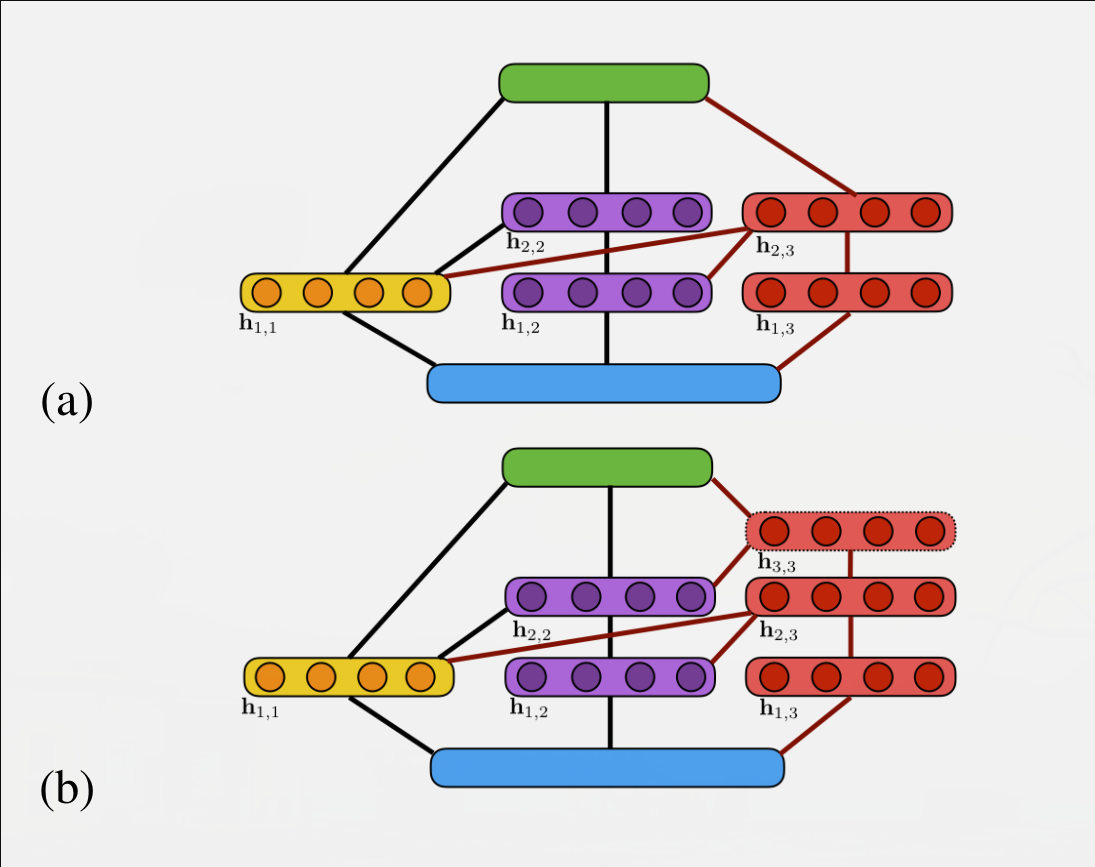
\includegraphics[width=0.5\textwidth]{schema.png}
	% \caption{Les deux sous réseaux candidats générés à l'étape $3$ (en rouge), un de profondeur $k=2$ comme le sous réseau choisi à l'étape précédente (en bleu), et un de profondeur $k=3$ qui augmente la profondeur générale de $1$. Ce sont ces deux réseaux AdaNets potentiels qui vont être évalués}
	\caption{Both of the candidate networks generated at step \(3\) (red), one of them with a depth of \(2\) (a), like the previously selected sub-network (blue), and one of depth \(3\) that adds a depth level. Both of these potential AdaNet networks are the ones that will be evaluated}
	\label{candidateModels}
\end{figure}

% \section{Choix lors des expérimentations}
\section{Experimental choices}
% \subsection{Choix du dataset}
\subsection{Dataset choice}

	% Une parmi deux expérimentations à reproduire était au choix :
	\paragraph{} One of two experiments on different datasets had to be chosen:
	\begin{itemize}
		\item CIFAR-10 dataset
		\item Criteo dataset
	\end{itemize}

	% Le choix s'est porté sur la taille du jeu de données à traiter. Si l'on ne retient que deux classes à traiter, CIFAR contient moins de 10000 éléments par classe tandis que le dataset Criteo contient 30 millions de lignes pour le set d'entraînement.
	The choice was made on the size of the respective datasets. If we concentrate on a given binary classification task, CIFAR has \(\approx 10000\) samples per class, whereas the Criteo dataset has \(30\) million. Therefore, considering our limited resources, the choice was made to work on the CIFAR-10 dataset.

% \subsection{Choix du langage et de l'API}
\subsection{API choice}
	% On programme sous \texttt{Python} et on utilise l'API \texttt{Keras} pour sa syntaxe simple et sa très grande modularité. Le backend utilisé est \texttt{Tensorflow} mais cela n'a aucune influence sur le code dans \texttt{Keras}.
	\paragraph{} All programs were coded in \texttt{Python} using the \texttt{Keras} API for neural networks because of it's simple syntax and high modularity. The \texttt{TensorFlow} backend is used but it has no influence on the \texttt{Keras} code.

% \subsection{Imprécisions du papier}
\subsection{Ambiguities in the paper}
% \subsubsection{Gestion des tenseurs multiples en entrée}
\subsubsection{Multiple input tensors management}
\label{subsec:mult}

% On ne sait pas si lorsqu'une couche reçoit les entrées de plus d'une autre couche les tenseurs sont soit :
% \begin{itemize}
% 	\item juxtaposés (fonction \texttt{concatenate})
% 	\item sommés (fonction \texttt{add})
% \end{itemize}
\paragraph{}When a layer, is connected (on the input side), to more than one layer of the other sub-networks, it is unclear if the tensors are: \medskip
\begin{itemize}
	\item juxtaposed (\texttt{concatenate} function)
	\item added (\texttt{add} function)
\end{itemize}

% \subsubsection{Régularisation des sous réseaux}
\subsubsection{Sub-network regularization}
% On ne sait pas explicitement si les sous réseaux sont régularisés à l'aide d'une norme $L_{1}$ ou $L_{2}$. L'utilisation du terme $\lambda$ nous fait choisir la norme $L_{1}$. On ne sait pas non plus si c'est la loss qui est régularisée ou les poids lors de l'apprentissage. On choisit de régulariser avec une norme $L_{1}$ les poids de chaque couche des sous réseaux ainsi que la couche de sortie.
\paragraph{} It is not explicitly stated wether the sub-networks are regularized using an \(L_1\) or \(L_2\) norm. The usage of \(\lambda\) term leads us to believe that an \(L_1\) norm was used. It is also unclear wether it is the loss function or the weights during training that are regularized. We have chosen to the weights of each layer of the sub-networks as well as the general output layer with an \(L_1\) norm.

% \section{Choix pour l'implémentation}
\section{Implementation choices}
% \subsection{Traitement des données en entrée}
\subsection{Input data pre-processing}
% Pour traiter les images en dehors d'un réseau de convolution, on vectorise celles-ci en un vecteur de longueur $width*height*3$
\paragraph{}To be able to use images outside of a Convolutional Neural Network framework, we vectorize the images to vector of size \(width*height*3\)

% \subsection{Architecture des couches d'entrée et de sortie}
\subsection{Input and output layers architecture}
\begin{itemize}
	% \item La couche d'entrée est de taille $width*height*3$ soit 3072 pour les images de CIFAR-10
	\item The input layer is of size \(width*height*3\), which is equal to \(3072\) in the case of CIFAR-10.
	% \item La couche de sortie contient un unique neurone et une activation sigmoïde, la classification étant binaire
	\item  The output layer is composed of a single neuron with a sigmoid activation function, since the classification task is binary.
\end{itemize}

% \subsection{Génération des sous réseaux}
\subsection{Sub-network generation}
% Nous choisissons de générer les sous réseaux aléatoirement. Chaque couche est connectée à la précédente du même sous réseau, mais les connexions avec les couches de niveau inférieur des autres sous réseaux est aléatoire.
\paragraph{} We chose to generate the sub-networks randomly. Each layer is connected to the preceding layer in it's own sub-network, however connections to the lower layers in previously selected sub-networks are made randomly.

% \subsection{Fonction objectif}
\subsection{Objective function}
\label{subsec:fobj}
\begin{multline*}
F_t(\mathbf{w,h})=\frac{1}{m}\sum^m_{i=1}\Phi(1-y_if_{t-1}(x_i)-y_i\mathbf{w\cdot h}(x_i))\\
+ \mathcal{R}(\mathbf{w,h})
\end{multline*}
% Avec $x_i$ les exemples d'entraînement, $y_i$ les réponses attendues, $m$ le nombre d'exemples,$\mathbf{w}$ les poids associés au sous réseau candidat $\mathbf{h}$ et $\Phi$ la fonction exponentielle. Le terme $\mathcal{R}(\mathbf{w,h})$ est un terme de régularisation qui est laiss\'e à $0$ lors des expérimentations.
\(x_i\) being the training samples, \(y_i\) their labels, \(m\) the number of training samples, \(\mathbf{w}\) the weights of the candidate sub-network \(\mathbf{h}\) and \(\Phi\) the exponential function. \(\mathcal{R}(\mathbf{w,h})\) is a regularization term left at \(0\) during experimentation.

\bigskip

% On interprète cette formule avec les conditions ci-dessus comme :
We interpret the formula as the following one:
\begin{multline*}
F_t(\mathbf{h})=\\
\frac{1}{m}\sum^m_{i=1}\exp(1-y_i \cdot pred_{t-1}(x_i)-y_i \cdot pred_{t-1 + \mathbf{h}}(x_i))
\end{multline*}

% \section{Implémentation pratique}
\section{Practical implementation}
% \paragraph{}Nous avons tenté d’être le plus fidèle possible à l’implémentation du papier. Nous avons du prendre quelques décisions cependant lorsque le papier n’était pas explicite sur la méthode utilisée.
\paragraph{}We have tried to be as faithful as possible with regrads to the implementation in the paper. We had to make some decisions however, when the paper did not explicitly state what method was used.

% \subsection{Génération et sélection des sous réseaux}
\subsection{Generation and selection of sub-networks}
% \paragraph{}Nous fournissons un paramètre à l'algorithme qui permet de spécifier combien de sous modèles candidats sont générés \`a chaque itération avec un paramètre \emph{reps}. Étant donne que dans le papier il n'y a que deux types de sous-réseaux générés (même profondeur ou profondeur +1) nous avons fait le choix de générer des sous réseaux de même profondeur que le réseau du pas de temps précédent pour les $\frac{reps}{2}$ premières itérations et des sous réseaux plus profonds pour les itérations suivantes.
\paragraph{}We give the algorithm a \textit{reps} parameter, allowing us to specify how many candidate sub-networks are generated a each iteration. Seeing as there are only 2 types of sub-networks generated (equal depth or depth + 1), we have chosen to generate same depth sub-networks for the \(\frac{reps}{2}\) first generation steps, and deeper sub-networks for the remaining generation steps.

% \paragraph{}Les connexions entre les différentes couches suivent les règles de connectivité décrites plus haut, c'est \`a dire dernière couche du sous réseau reliée à la couche de sortie, première couche du sous réseau reliée à la couche d’entrée et toutes les couches internes sont reliées entre-elles au sein d'un même sous réseau. La variabilité entre les sous réseaux candidats apparaît dans la connectivité entre les sous réseaux candidats. Pour chaque couche du sous-réseau candidat considéré, un nombre aléatoire de connexions aux sous couches de profondeur inférieure de 1 parmi les sous réseaux générés aux pas de temps précédents, est sélectionné.
\paragraph{}Connections between the different layers follow the connectivity ules laid out earlier, that is to say: the last layer of the sub-network is connected to the output layer, the first layer of the sub-network is connected to the input layer and the intermediary layers are connected to each other within a sub-network. Variability between the different candidate sub-networks lies in their connectivity to the previously selected sub-networks. For each layer of depth \(k\) of the considered candidate sub-network, a random number of connections to the layers of depth \(k-1\) of previously selected sub-networks are established.

% \paragraph{}Le nombre de neurones par sous couche des sous-réseaux candidats est déterminé par un paramètre fix\'e au début de l'algorithme. Donc toute la variabilité entre les candidats vient du nombre de connexions aux sous-réseaux précédents et au changement de profondeur.
\paragraph{}The number of neurons by layer is determined at the beginning of the algorithm by a parameter. So all of the variability come from the random connections.

% \paragraph{}Tous les sous-réseaux candidats sont insérés dans le réseau adanet de l’étape précédente pour être évalués, après entraînement, sur un set de test, selon la fonction objective définie en \ref{subsec:fobj}. Le résultat de la fonction objective le plus bas est mis en mémoire ainsi que le modèle adanet correspondant, et mis à jour si besoin à chaque évaluation de candidat. A la fin de l’évaluation des candidats le meilleur réseau est sauvegard\'e sur le disque et utilise comme modèle de base pour l’étape suivante.
\paragraph{}All the candidate sub-networks are inserted into the AdaNet network of the previous step to be evaluated on a test set, after training, using the objective function defined in \ref{subsec:fobj}. The lowest result of this function is stored as well as the corresponding AdaNet network, and updated if a better candidate is found at subsequent steps. At the end of the evaluation of all candidates, the best AdaNet model is saved to diskand used as the base model for the next iteration of the algorithm.

% \subsection{Implémentation de la gestion d’entrées multiples}
\subsection{Multiple input management implementation}
% \paragraph{}Comme dit dans la partie \ref{subsec:mult}, il n'est pas dit dans le papier, comment la gestion du nombre de neurones entrant variable pour certaines couches. Si on concatène les tenseur des couches entrantes on change la taille d’entrée de la couche supérieure. Ceci pose un problème lors du chargement des poids du modèle adanet de l’étape précédente puisque le tenseur de poids sauvegardes et le nouveau tenseur ne font plus la même taille. Une solution que nous avons utilisée est de ne pas charger les poids précédents pour ces couches de concaténation. cependant cela peut faire perdre en performance. Nous avons donc préféré sommer les tenseurs entrants et garder les poids de l’itération précédente.
\paragraph{}As mentionned in \ref{subsec:mult}, it is not stated in the paper how multiple input connections to a layer are managed. If we concatenate all the input tensors the size of the input tensor for the output layer changes over iterations. This can lead to problems when loading weights from a previous network, since the saved tensor and the new one are not the same size. One solution would be to not save the weights for these concatenation layers, however this could lead to a decrease in performance. We have therefore chosen to add the input tensors for such layers and keep the existing weights.

% \subsection{Problème de flexibilité}
\subsection{Flexibility problems}
% \paragraph{} Puisque la structure change constamment au fur et à mesure des itérations on ne peut pas se contenter de sauvegarder les modèles directement au disque puisque l'on ne peut pas changer les modèles une fois qu'ils sont compil\'es. Pour pouvoir passer outre ce problème nous avons sauvegard\'e la structure exacte du modèle dans un dictionnaire et on reconstruit le modèle \`a partir de ce dictionnaire à chaque itération. Une fois construit on charge les poids de l'ancien modèle dans les couches qu'il a en commun avec le nouveau à chaque itération le dictionnaire correspondant au meilleur modèle est simplement s\'erialisable puisque ça n'est que du texte.
\paragraph{} Since the structure of the network is constantly changing, we cannot save the models directly to disk, since once compiled in \texttt{Keras} they are not modifiable. To be able to bypass this issue, we store the exact topology of the best model in a dictionnary at each iteration. This dictionnary is then used to rebuild the network from scratch at the next iteration. Once reconstructed, we load the weights of the previous model in the common layers between \(f_t\) and \(f_{t-1}\). The dictionnary is easily serializable since it is only text.

% \subsection{Condition d’arrêt}
\subsection{Stop condition}
% \paragraph{}Dans le papier il est dit que l'algorithme s’arrête lorsque l'ajout d'un nouveau sous-réseau ne fait pas diminuer sa fonction objectif. Au regard de nos puissances limitées de calcul nous avons fait le choix de s’arrêter lorsque la diminution de la fonction objective passe sous un certain seuil. L’entraînement des différents sous-réseaux est aussi soumis à une condition similaire d’arrêt lorsque l'erreur de classification sur un jeu de validation ne diminue plus.
\paragraph{}In the paper, it is stated that the algorithm stops when the addition of a new sub-network doesn't reduce the objective function. Cosidering our limited computing resources, we made the choice to stop when the decrease in the objective function was under a certain threshold. The training of the various sub-networks was also submitted to a similar stop condition when the classification error did not decrease anymore.

% \section{Résultats}
\section{Results}
% \paragraph{}Nous n'avons pas pu refaire toutes les optimisations d'hyper-paramètres qui ont été faites dans le papier, donc nous avons simplement choisi un jeu d'hyper-paramètres pour nos expérimentations:
\paragraph{} We were unable to redo all the hyperparameter optimizations that were done in the paper, therefore we have chosen a set of hyperparameters for our experiments:

\begin{itemize}
%   \item $n = 150$, le nombre de neurones dans chaque couche
  \item \(n=150\), the number of neurons in each layer
%   \item $\lambda = 0.000001$, le paramètre de normalisation
  \item \(\lambda = 10^{-6}\), the normalization parameter
%   \item $\eta = .001$, le taux d'apprentissage
  \item \(\eta=10^{-3}\), the learning rate
%   \item $T = 10$, le nombre de répétitions
  \item \(T=10\), the number of iterations
%   \item $reps = 5$ le nombre de sous-réseaux générés a chaque étape
  \item \(reps=5\), the number of sub-networks generated at each iteration.
\end{itemize}

% \paragraph{}Nous avons ensuite exécuté notre algorithme sur différents jeux de données binaires (les mêmes que ceux du papier), mesur\'e leur précision de classification sur un jeu de test et sur 10 exécutions pour avoir une performance moyenne et un écart-type. Il est à noter que le set CIFAR-10 est déjà séparé en un set de test et d'entraînement. On obtient alors les résultats de la table \ref{table:res}
\paragraph{}We then executed our algorithm on different binary classification tasks extracted from the CIFAR-10 dataset (identical to the ones used in the paper), measured the classification accuracy on a test set 10 times, to have an average performance as well as standard deviation. It is important to note that CIFAR-10 is already separated in training and testing sets. The results are shown in Table~\ref{table:res}.

\begin{table*}[t]
	\centering
	  \begin{tabular}{c c c}
			\toprule
			  classification task &our results &paper results \\
		  \midrule
			\texttt{deer-truck} & $\mathbf{0.2741\pm0.0391}$ & $0.9372 \pm 0.0082$ \\
			\texttt{deer-horse} & $\mathbf{0.8731 \pm0.0097}$ & $0.8430 \pm 0.0076$ \\
			\texttt{automobile-truck} & $\mathbf{0.2521 \pm0.0204}$ & $0.8461 \pm 0.0069$\\
		  \texttt{cat-dog} & $\mathbf{ 0.3085\pm0.0449}$ & $0.6924 \pm 0.0129$\\
		  \texttt{dog-horse} & $\mathbf{0.5711 \pm0.0172}$ & $0.8350 \pm 0.0089$\\
			\bottomrule
	  \end{tabular}
	  \caption{Comparison of classification accuracy between our implementation and paper implementation}
	  \label{table:res}
  \end{table*}

% \paragraph{} Les résultats sont très variables en fonction des couples. Cela s'explique par le fait qu'aucune optimisation des hyper-paramètres n'a été faite. Ainsi, à la faveur des choix arbitraires que l'on a fait on peut se retrouver tant avec de très bon résultats (deer-horse) qu'avec de mauvais résultats.
\paragraph{} The results vary a lot between different tasks. This can be explained by the fact that no hyper-parameter optimization was done. Therefore the chosen hyper-parameters favor certain tasks \textit{(deer-horse)} and lead to poor results for others.

% \begin{table*}[t]
%   \centering
%     \begin{tabular}{c c c}
%       	\toprule
%        	 jeu de données &résultat de notre version &résultat papier \\
%         \midrule
%       	\texttt{deer-truck} & $\mathbf{0.2741\pm0.0391}$ & $0.9372 \pm 0.0082$ \\
%       	\texttt{deer-horse} & $\mathbf{0.8731 \pm0.0097}$ & $0.8430 \pm 0.0076$ \\
%       	\texttt{automobile-truck} & $\mathbf{0.2521 \pm0.0204}$ & $0.8461 \pm 0.0069$\\
%         \texttt{cat-dog} & $\mathbf{ 0.3085\pm0.0449}$ & $0.6924 \pm 0.0129$\\
%         \texttt{dog-horse} & $\mathbf{0.5711 \pm0.0172}$ & $0.8350 \pm 0.0089$\\
%       	\bottomrule
%     \end{tabular}
%     \caption{Comparaison des précisions de classification entre la version du papier et la notre}
%     \label{table:res}
% \end{table*}


\section{Conclusion}
% Nous avons essayé dans ce projet de reproduire les résultats d'Adanet. Nous avons été contraints de faire des choix, notamment sur la génération des sous réseaux et nous avons du nous priver d'optimisation des hyper-paramètre (nécessité d'implémenter en plus une méthode sophistiquée). De ce fait, les résultats que nous avons obtenus sont, exception faite pour deer-horse, nettement moins bons que ceux obtenus dans le papier. Certains des résultats que nous avons obtenus (deer-truck, automobile-truck et cat-dog) semblent biais\'es puisque l’on obtient des précisions inférieures a $50\%$.
% Dans tous les cas, des performances nettement meilleures que celles obtenues dans le papier peuvent être obtenues via du transfert learning (précision supérieure à 90\%). Ceci ne montre pas clairement l'intérêt de cette méthode très nécessiteuse de calculs (génération d'un grand nombre de sous réseaux). Cependant, si l'on ne dispose pas d'un modèle entraîné pour faire de l'apprentissage par transfert, alors cette approche peut être intéressante.

\paragraph{}We have strived to reproduce the results from the AdaNet paper. However we were forced to make some choices, notably on the sub-network generation steps, as well as forego any hyper-parameter optimization (it would have required implementation of an additional sophisticated method). Therefore, the results we have obtained, apart from the deer-horse classification task, are significantly lower than the one found in the paper. Certain results (deer-truck, automobile-truck and cat-dog) seem biased since we have obtained accuracies lower than \(50\%\) with balanced classes. In anycase, better results can be obtained with transfer learning (accuracy \(> 90\%\)), so the benefits of this method are unclear. This method is very costly in computing time (due to the generation of a large number of sub-networks). However if we do not have a pre-trained network this method might yield results more quickly than when using convolutional  neural networks, and could be interesting.

\end{document}
